%%% NEJM2004.tex --- 
%% Version: $Id: NEJM2004.tex,v 0.0 2012/05/09 02:41:44 tangboyun Exp$
%% Copyright : (c) 2012 Boyun Tang
%% License : BSD-style
\documentclass{standalone}
\usepackage{tikz}
\usetikzlibrary{mindmap,shadows,shapes.arrows,shapes.geometric,shapes.misc,matrix,arrows,positioning,calc,decorations.pathreplacing,petri}
\usepackage{graphicx}
\usepackage{times}
\usepackage{xcolor}

\begin{document}
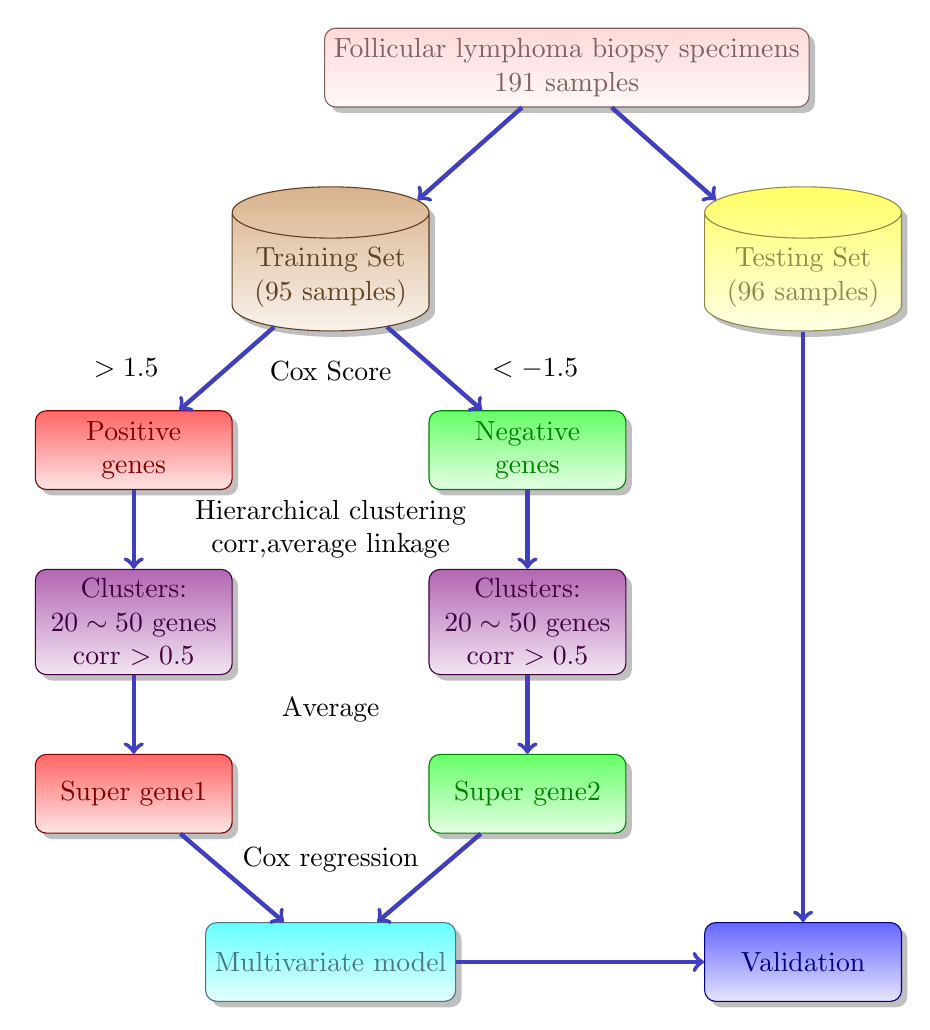
\begin{tikzpicture}[
  every node/.style={minimum width=2.5cm,minimum height=1cm,align=center,},%
  dr/.style={drop shadow},%
  e/.style={->,ultra thick,rounded corners,draw=blue!50!gray},%
  cl/.style={cylinder,aspect=.3,shape border rotate=90,},%
  re/.style={rounded corners,},%
  r/.style={top color= red!60,bottom color= red!10,draw=red!50!black,%
    text=red!50!black,},%
  g/.style={top color= green!60,bottom color= green!10,draw=green!50!black,%
    text=green!50!black,},%
  b/.style={top color= blue!60,bottom color= blue!10,draw=blue!50!black,%
    text=blue!50!black,},%
  br/.style={top color= brown!60,bottom color= brown!10,draw=brown!50!black,%
    text=brown!50!black,},%
  v/.style={top color= violet!60,bottom color= violet!10,draw=violet!50!black,%
    text=violet!50!black,},%
  o/.style={top color= orange!60,bottom color= orange!10,draw=orange!50!black,%
    text=orange!50!black,},%
  ye/.style={top color= yellow!60,bottom color= yellow!10,draw=yellow!50!black,%
    text=yellow!50!black,},%
  p/.style={top color= pink!60,bottom color= pink!10,draw=pink!50!black,%
    text=pink!50!black,},%
  c/.style={top color= cyan!60,bottom color= cyan!10,draw=cyan!50!black,%
    text=cyan!50!black,},%
  ]
  \node (sample) [re,p,dr%
  ] {Follicular lymphoma biopsy specimens\\191 samples};

  \node (train) [cl,below=of sample,xshift=-3cm,br,dr%
  ] {Training Set\\(95 samples)};

  \node (test) [cl,below=of sample,xshift=3cm,ye,dr%
  ] {Testing Set\\(96 samples)};
  
  \node (pg) [re,below=of train,xshift=-2.5cm,r,dr
  ] {Positive\\genes};
  \node (ng) [re,below=of train,xshift=2.5cm,g,dr
  ] {Negative\\genes};

  \node (clp) [re,below=of pg,v,dr
  ] {Clusters: \\$20\sim 50$ genes\\corr $> 0.5$};
  \node (cln) [re,below=of ng,v,dr%
  ] {Clusters: \\$20\sim 50$ genes\\corr $> 0.5$};
  \node (sg1) [re,below=of clp,r,dr%
  ] {Super gene1};
  \node (sg2) [re,below=of cln,g,dr%
  ] {Super gene2};
  \node (model) [re,below=of train,yshift=-6.5cm,c,dr%
  ] {Multivariate model};
  \node (valid) [re,below=of test,yshift=-6.5cm,b,dr%
  ] {Validation};

  \draw [e] (sample) -- (train);
  \draw [e] (sample) -- (test);
  \draw [e] (train) -- (pg) node [midway,left] {$>1.5$};
  \draw [e] (train) -- (ng) node [midway,right] {$< -1.5$};
  \draw [e] (pg) -- (clp);
  \draw [e] (ng) -- (cln);
  \draw [e] (clp) -- (sg1);
  \draw [e] (cln) -- (sg2);
  \draw [e] (sg1) -- (model);
  \draw [e] (sg2) -- (model);
  \draw [e] (model) -- (valid);
  \draw [e] (test) -- (valid);

  \node [below=of train,yshift=1cm] {Cox Score};
  \node [below=of train,yshift=-1cm] {Hierarchical clustering\\corr,average linkage};
  \node [below=of train,yshift=-3.3cm] {Average};
  \node [below=of train,yshift=-5.2cm] {Cox regression};
\end{tikzpicture}

\end{document}

%%% Local Variables: 
%%% TeX-master: "../../LaTeX/"
%%% End: 
